\documentclass[a4paper, 12pt]{report}
% Allows writing the document in english.
\usepackage[francais]{babel}
% Allows to use images.
\usepackage{graphicx}
% Provides hyperlinks within the document.
\usepackage{enumitem}
% Adds space between paragraphs.
\usepackage{parskip}
% Supports Text Companion fonts (necessary for gensymb).
\usepackage{textcomp}
\usepackage{array}
\usepackage{multicol}
% Better tabular
\usepackage{tabularx}
% Allows to use colors.
\usepackage{xcolor}
\usepackage[margin=4cm]{geometry}
\usepackage{varwidth}
% Euro
\usepackage{eurosym}
\usepackage{amsmath}
\usepackage{fontspec}
\usepackage[T1]{fontenc}
\usepackage{lmodern}


\usepackage{gensymb}

% Default fixed font does not support bold face
\DeclareFixedFont{\ttb}{T1}{txtt}{bx}{n}{12} % for bold
\DeclareFixedFont{\ttm}{T1}{txtt}{m}{n}{12}  % for normal

\setcounter{tocdepth}{3}

% Custom colors
\usepackage{color}
\definecolor{deepblue}{rgb}{0,0,0.5}
\definecolor{deepred}{rgb}{0.6,0,0}
\definecolor{deepgreen}{rgb}{0,0.5,0}

\usepackage{listings}
\usepackage{subfigure}
\usepackage[
    type={CC},
    modifier={by-nc-nd},
    version={4.0},
]{doclicense}

\usepackage[colorlinks=true,urlcolor=black,linkcolor=black]{hyperref}

% Replace Table by Tableau
\addto\captionsfrench{\def\tablename{Tableau}}
% New columns types
% Left
\newcolumntype{L}{>{\raggedright\arraybackslash}X}
% Center
\newcolumntype{C}{>{\centering\arraybackslash}X}
% Right
\newcolumntype{R}{>{\raggedleft\arraybackslash}X}

% Add more space before and after table
\newenvironment{centerspace}{\setlength{\topsep}{1ex}\center}{\endcenter}
% Sets the color of gray.
\newcommand{\gray}{\rowcolor[gray]{.90}}
% Allows to draw lines.
\newcommand{\HRule}{\rule{\linewidth}{0.5mm}}
% Uses the arabic numerals for sections.
\renewcommand{\thesection}{\arabic{section}}

% Width of text.
\addtolength{\textwidth}{2cm}
% Odd page left margin.
\addtolength{\oddsidemargin}{-1cm}
% Height of main text.
\addtolength{\textheight}{2cm}
% Removes indentation.
\setlength\parindent{0pt}
% Indicates overflow words.
\setlength{\overfullrule}{10pt}
% Height of items.
\setitemize{itemsep=1em}

%%%%********************************************************************
% fancy quotes
\definecolor{quotemark}{gray}{0.7}
\makeatletter
\def\fquote{%
    \@ifnextchar[{\fquote@i}{\fquote@i[]}%]
           }%
\def\fquote@i[#1]{%
    \def\tempa{#1}%
    \@ifnextchar[{\fquote@ii}{\fquote@ii[]}%]
                 }%
\def\fquote@ii[#1]{%
    \def\tempb{#1}%
    \@ifnextchar[{\fquote@iii}{\fquote@iii[]}%]
                      }%
\def\fquote@iii[#1]{%
    \def\tempc{#1}%
    \vspace{1em}%
    \noindent%
    \begin{list}{}{%
         \setlength{\leftmargin}{0.1\textwidth}%
         \setlength{\rightmargin}{0.1\textwidth}%
                  }%
         \item[]%
         \begin{picture}(0,0)%
         \put(-15,-5){\makebox(0,0){\scalebox{3}{\textcolor{quotemark}{``}}}}%
         \end{picture}%
         \begingroup\itshape}%
 %%%%********************************************************************
 \def\endfquote{%
 \endgroup\par%
 \makebox[0pt][l]{%
 \hspace{0.8\textwidth}%
 \begin{picture}(0,0)(0,0)%
 \put(15,15){\makebox(0,0){%
 \scalebox{3}{\color{quotemark}''}}}%
 \end{picture}}%
 \ifx\tempa\empty%
 \else%
    \ifx\tempc\empty%
       \hfill\rule{100pt}{0.5pt}\\\mbox{}\hfill\tempa,\ \emph{\tempb}%
   \else%
       \hfill\rule{100pt}{0.5pt}\\\mbox{}\hfill\tempa,\ \emph{\tempb},\ \tempc%
   \fi\fi\par%
   \vspace{0.5em}%
 \end{list}%
 }%
 \makeatother

 %%%% ********************************************************************

% Starts roman numbering (trick to not numbering the first pages).
\pagenumbering{roman}

\begin{document}
\renewcommand{\bibname}{Références}
\begin{center}
  
  \begin{figure}[!h]
    \centering
    
\includegraphics[width=0.25\textwidth]{textures/logo/heh_bw.eps}    
  \end{figure}

  \textsc{\LARGE Serveur Linux} \\ [0.5cm]
  \textsc{\Large Installation et configuration} \\ [0.5cm]

  \textsc{\large 2\up{ème} Bachelier en Informatique} \\ [0.2cm]

  \begingroup
  \fontfamily{pag} \selectfont 

  \HRule \\ [0.4cm] {
    \huge Projet Linux \\ [0.2cm] 
  }
  \HRule \\ [1.3cm]
  \endgroup

  \begin{minipage}[t]{0.4 \textwidth} 
    \begin{flushleft} 
      \large \emph{Auteur:} \\ 
      Terencio \textsc{Agozzino}
    \end{flushleft} 
  \end{minipage}
  % 
  \begin{minipage}[t]{0.4 \textwidth}
    \begin{flushright} 
      \large \emph{Auteur :} \\ 
      Alexandre \textsc{Ducobu}
    \end{flushright} 
  \end{minipage}

  \vspace{1.5cm}

  \begin{minipage}[t]{0.4 \textwidth}
    \begin{center} 
      \large \emph{Enseignants:} \\ 
      Antoine \textsc{Malaise} \\
      Julien \textsc{De Bodt}
    \end{center} 
  \end{minipage}

  \vspace{1cm}

  \begin{figure}[!h]
    \centering
    
\includegraphics[scale=0.08]{textures/logo/technical_bw.pdf}
  \end{figure}
  
  \vspace{0.5cm}

  Année académique 2016 - 2017
\end{center}

\thispagestyle{empty}

\newpage
\newpage
\thispagestyle{empty}
\setcounter{page}{0}
\null
\newpage
\begin{center}
  
\includegraphics[scale=0.12]{textures/logo/heh.pdf}

  \vspace{1cm}

  \textsc{\LARGE Serveur Linux} \\ [0.5cm]
  \textsc{\Large Installation et configuration} \\ [0.5cm]

  \textsc{\large 2\up{ème} Bachelier en Informatique} \\ [0.2cm]

  \begingroup
  \fontfamily{pag} \selectfont 

  \HRule \\ [0.4cm] {
    \huge Projet Linux \\ [0.2cm] 
  }
  \HRule \\ [1.3cm]
  \endgroup

  \begin{minipage}[t]{0.4 \textwidth} 
    \begin{flushleft} 
      \large \emph{Auteur:} \\ 
      Terencio \textsc{Agozzino}
    \end{flushleft} 
  \end{minipage}
  % 
  \begin{minipage}[t]{0.4 \textwidth}
    \begin{flushright} 
      \large \emph{Auteur :} \\ 
      Alexandre \textsc{Ducobu}
    \end{flushright} 
  \end{minipage}

  \vspace{1.5cm}

  \begin{minipage}[t]{0.4 \textwidth}
    \begin{center} 
      \large \emph{Enseignants:} \\ 
      Antoine \textsc{Malaise} \\
      Julien \textsc{De Bodt}
    \end{center} 
  \end{minipage}

  \vspace{1cm}

  
\includegraphics[scale=0.08]{textures/logo/technical.pdf}

  \vspace{0.5cm}

  Année académique 2016 - 2017
\end{center}

\thispagestyle{empty}

\newpage
\newpage
\thispagestyle{empty}
\setcounter{page}{0}
\null
\newpage
%\newpage
%\input{src/thanks}
\newpage
\mbox{~}
\vfill
Ce document est mis à disposition selon les termes de la licence Creative
Commons “\href{https://creativecommons.org/licenses/by-nc-nd/4.0/}{Attribution
- Pas d'utilisation commerciale 4.0 International}”.

\begin{center}
  
\includegraphics[scale=1]
    {textures/images/license/license.pdf}
\end{center}
\setcounter{page}{0}
\thispagestyle{empty}

\newpage
\pagenumbering{arabic}
\tableofcontents
\newpage
\section{Présentation générale du projet}
\label{sec:pres-gener-du}


\subsection{Introduction}
\label{sec:introduction}

Dans le cadre de ce projet, il nous a été demandé d'administrer un serveur sous
Linux. \\
Le choix de la distribution ainsi que la gestion des sauvegardes est libre et
devra être justifié. \\

Le serveur devra contenir :

\begin{itemize}
    \item un partage \textbf{NFS} qui permettra aux utilisateurs du réseaux local d'y stocker des fichiers;
    \item un partage \textbf{Samba} permettra aux utilisateurs Windows d'accéder à ce même partage;
    \item un serveur \textbf{Web}, \textbf{FTP}, \textbf{MySQL} et \textbf{DNS} qui permettra un hébergement multi-utilisateurs;
    \begin{itemize}
        \item[$\bullet$] le FTP permettra à chaque utilisateur d'accéder à son dossier Web;
        \item[$\bullet$] il faudra créer une zone dans le DNS pour nos sites;
        \item[$\bullet$] le DNS fera également office de DNS cache pour le réseau local;
    \end{itemize}
    \item un \textbf{serveur de temps} pour que les machines du
    réseau local puissent se synchroniser;
    \item une connexion en \textbf{SSH} au serveur.
\end{itemize}


\newpage


\subsection{Déontologie}
\label{sec:déontologie}

En tant qu'administrateurs du serveur, nous serons tenus de suivre de nombreuses
règles telles que :

\begin{itemize}
    \item la documentation des actions entreprises sur le serveur;
    \item l'automatisation des installations et configurations au travers de scripts;
    \item la sécurité : mise en place de mots de passe forts, du SSH, etc.
    \item la vigilance et la prévoyance, par exemple par la mise en place de
    sauvegardes avant et après chaque changements sur le serveur;
    \item le contrôle du bon fonctionnement de chaque élément.
\end{itemize}


\subsection{Sécurité}
\label{sec:securite}

Du côté de la sécurité, nous avons quelques contraintes reprises ci-dessous :

\begin{itemize}
    \item mise en place d'une politique utilisateur;
    \item mise en place de quotas;
    \item partitionnement et gestion du disque \textit{(\textbf{LVM} et
    \textbf{RAID})};
    \item mise en place d'une stratégie de sauvegarde;
    \item désactivation des éléments inutiles et des mises à jours;
    \item mise en place d'un antivirus, d'un firewall, etc.
\end{itemize}

%%% Local Variables:
%%% mode: latex
%%% TeX-master: t
%%% End:

\newpage
\chapter*{Installation} %On garde ?
\label{cha:installation}

\section{Choix}
\label{sec:choix}

\subsection{Distribution}
\label{sec:distribution}

Notre choix de la distribution s'est naturellement porté sur Debian, pour ses
nombreux avantages. En voici quelques exemples :

\begin{itemize}
\item Large communauté : grâce à cela, les erreurs et problèmes rencontrés ont
  souvent plusieurs solutions connues et éprouvées.

\item Plusieurs architectures et noyaux : Debian supporte la majorité des
  architectures de processeurs comme AMD, Armel, i386, MIPS, etc. Elle supporte
  aussi de nombreux noyaux tels que FreeBSD et GNU Hurd.

\item Sécurité : vu que la distribution est open-source, cela signifie que les
  backdoors sont presque inexistantes. De surcroît, lorsqu'une faille de sécurité
  est détectée, celle-ci est rapidement corrigée par la communauté.

  En outre, Debian comprend de nombreux logiciels de sécurité tels que GPG (et
  PGP), SSH et autres.

\item Stabilité : nous savons que les serveurs doivent avoir le plus grand temps
d'accessibilité ($\approx$ 99.999\%). Sous Debian, il existe de nombreux exemples de
machines qui tournent sans arrêt pendant des années, mis à part lors de pannes
ou de mises à jour matérielles.

\item Système de paquets : grâce au système de paquets, les distributions Linux
ont la possibilité d'installer de nombreux logiciels par une seule ligne de
commande. Le système de paquets de Debian est l'outil central de mise à jour,
installation, suppression et recherche de paquets.
\end{itemize}

\newpage

De même, la distribution Debian est plus professionnel et celle-ci possède le
leadership depuis des années.

À titre d'information, depuis mai 2016, Ubuntu a les mêmes parts de marché que
Debian.

\begin{figure}[!h]
    \centering
    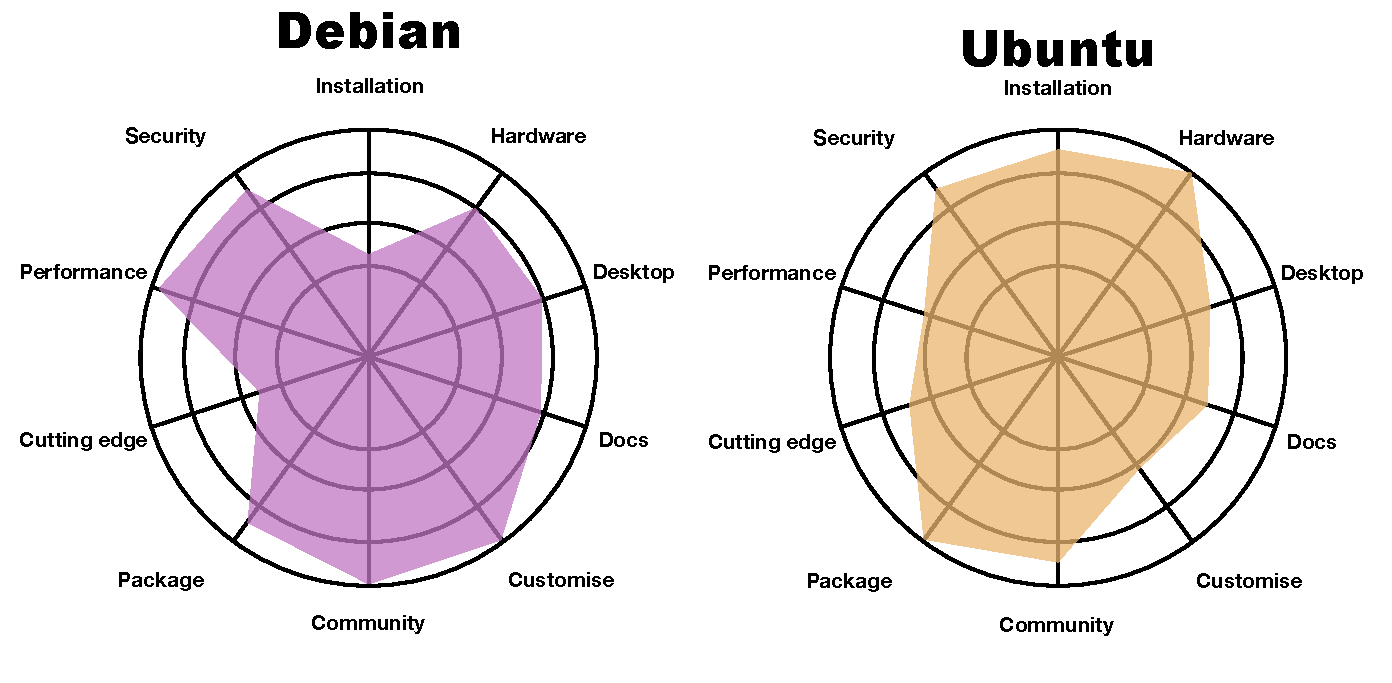
\includegraphics[scale=0.4]
    {textures/images/installation/DebianVsUbuntu.pdf}
    \caption{Différences entre Debian et Ubuntu}
     \label{fig:diff-debian-ubuntu}
  \end{figure}

Nous n'avons pas choisi Ubuntu pour les raisons suivantes :

\begin{itemize}
\item C'est un dérivé de Debian : de ce fait, un administrateur sachant
  configurer un serveur Debian pourra faciliter s'adapter au serveur Ubuntu.

\item Il vise le grand public et, de ce fait, est beaucoup moins utilisé
  dans le milieu professionnel.

\item Celui-ci est assez récent sur le marché du serveur.

\item Moins performant que Debian.
\end{itemize}

Concernant les autres distributions, CentOS est en baisse, mais reste au-dessus
de Red Hat et de Fedora qui, lui, est en chute libre.

\begin{figure}[h]
  \centering
  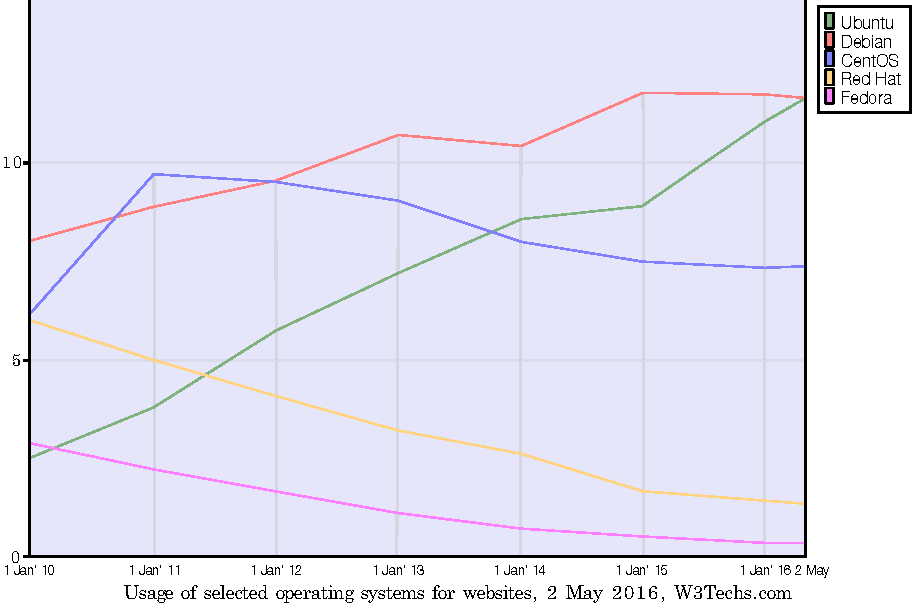
\includegraphics[scale=0.63]
  {textures/images/installation/distributions.pdf}
  \caption{Parts de marché des distributions Linux}
\end{figure}

\newpage

\subsection{Langue}
\label{sec:langue}

Pour le choix de la langue lors de l'installation, il a été préféré d'utiliser
l'anglais vu que la majorité des documentations et forums sont disponibles dans
cette langue. De plus, cela permet d'éviter une mauvaise traduction concernant
les nouvelles mises à jour et de toucher un plus large public possible.

\subsection{Noyau}
\label{sec:noyau}

Un noyau (monolithique) modulaire a été choisi afin de gérer les
modules. En effet, celui-ci facilite l'ajout et la suppression de modules à
chaud. Ces modules, pas toujours indispensables, peuvent être la source de
failles et de bugs.

\subsection{Partitionnement}
\label{sec:partitionnement}

Nous avons partitionné le disque de cette manière, avec un partition racine,
\textit{/boot}, et un groupe de volume LVM, \textit{VolGroup} : \\

\begin{center}
    \begin{table}[h]
        \begin{tabularx}{\linewidth}{|C|C|C|C|}
            \hline
            Label & Type & Taille (Mo) & Format \\
            \hline
            \hline
            /boot & primary & 512 & ext4 \\
            \hline
            VolGroup & logical & 20958 & lvm \\
            \hline
        \end{tabularx}

        \vskip .5cm

        \begin{tabularx}{\linewidth}{|C|C|C|C|}
            \hline
            LVsrv (/srv) & lvm & 6144 & ext4 \\
            %web et nfs
            \hline
            LVswap (/swap) & lvm & 4096 & swap \\
            \hline
            LVhome (/home) & lvm & 2048 & ext4 \\
            \hline
            LVroot (/root) & lvm & 2048 & ext4 \\
            \hline
            LVusr (/usr) & lvm & 2048 & ext4 \\
            \hline
            LVopt (/opt) & lvm & 2048 & ext4 \\
            \hline
            LVvar (/var) & lvm & 1024 & ext4 \\
            \hline
            LVtmp (/tmp) & lvm & 1024 & ext4 \\
            \hline
        \end{tabularx}
        \caption{Tableau du partitionnement \textit{(avec LVM)}}
        \label{tab:tableau-partitionnement}
    \end{table}
\end{center}

%%% Local Variables:
%%% mode: latex
%%% TeX-master: t
%%% End:

\newpage
\chapter*{Gestion}
\label{ch:gestion}


\section{Sauvegardes}
\label{subsec:sauvegardes}

Dans le milieu de l'entreprise, deux types de sauvegarde sont utilisées :
incrémentielle et différentielle.

La méthode de sauvegarde choisie est la différentielle, afin de restaurer les
données plus rapidement par rapport à la sauvegarde incrémentielle. De plus,
cette méthode est plus fiable, car seule la sauvegarde complète est nécessaire
pour reconstituer les données sauvegardées.

Il est à remarqué que la sauvegarde incrémentielle est plus économe en terme de
stockage.

Pour terminer, nous prévoyons d'effectuer une sauvegarde complète une fois
toutes les semaines.

\newpage


\section{Mise en œuvre}
\label{subsec:mise-en-œuvre)}




%%% Local Variables:
%%% mode: latex
%%% TeX-master: t
%%% End:

\newpage
\phantomsection
\nocite{*}
\addcontentsline{toc}{section}{Références}
\bibliographystyle{acm} 
\bibliography{bibli}
\newpage
\newpage
\thispagestyle{empty}
\setcounter{page}{0}
\null
\newpage
\end{document}
